%%%%%%%%%%%%%%%%%%%%%%%%%%%%%%%%%%%%%%%%%%%%%%%%%%%%%%%%%%%%%%%%%%%
%%% Documento LaTeX                                             %%%
%%%%%%%%%%%%%%%%%%%%%%%%%%%%%%%%%%%%%%%%%%%%%%%%%%%%%%%%%%%%%%%%%%%
% Título:   Apéndice A
% Autor:    Ignacio Moreno Doblas
% Fecha:    2014-02-01
% Versión:  0.5.0
%%%%%%%%%%%%%%%%%%%%%%%%%%%%%%%%%%%%%%%%%%%%%%%%%%%%%%%%%%%%%%%%%%%%

\pagestyle{fancy}
\fancyhead[LE,RO]{\thepage}
\fancyhead[RE]{Apéndice} %
\fancyhead[LO]{\nouppercase{\rightmark}}
%\fancyhead[RE]{Parte \thepart \rightmark} %

\chapterbegin{Funcionamiento de la placa auxiliar}
\label{chp:PlacaAux}
\minitoc

\section{Esquema}

\begin{figure}[h]
  \centering
    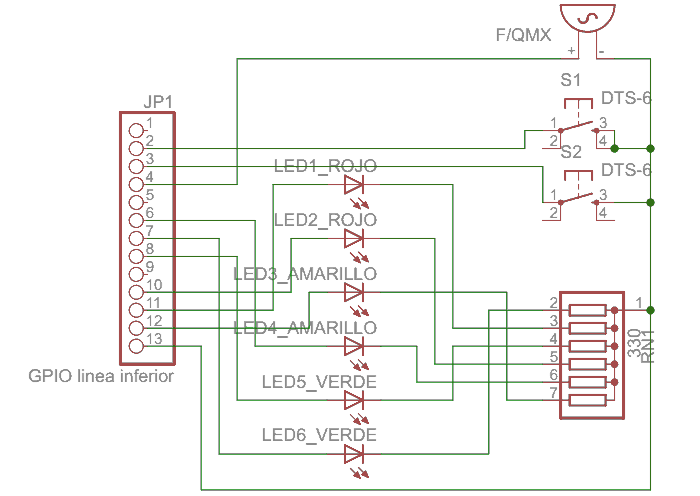
\includegraphics[width=14cm]{graphs/circuito.png}
  \caption{Esquema del circuito}
  \label{fig:circuito}
\end{figure}

Es un circuito sencillo y se puede montar en una protoboard sin
problemas, el esquema es el siguiente. Se conecta en la fila
inferior del conector GPIO, dejando libre la superior para el puerto
serie y otros propósitos.

\section{Pinout}

El puerto GPIO varía ligeramente dependiendo del modelo de Raspberry. En nuestro caso
la mayor diferencia está entre la revisión 1 y la 2, ya que el modelo B+ es compatible.
Al ser idénticos los primeros 26 pines, cualquier periférico diseñado para la revisión 2
es compatible con el modelo B+ (pero no al contrario).

La zona marcada con un recuadro verde es donde conectaremos nuestra placa auxiliar.

\begin{figure}[h]
  \centering
    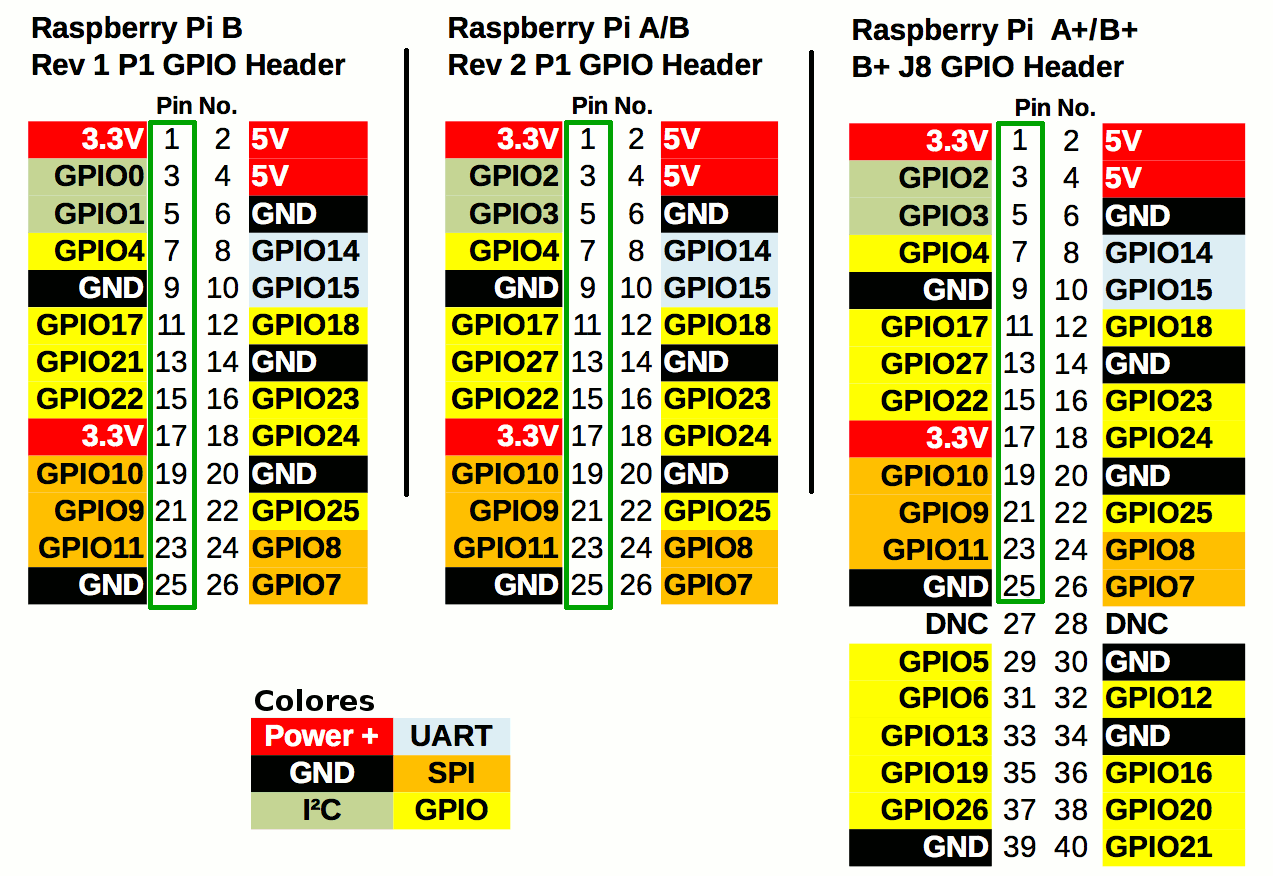
\includegraphics[width=14cm]{graphs/RaspberryGPIO.png}
  \caption{Pinout del puerto GPIO}
  \label{fig:pinout}
\end{figure}

\section{Correspondencia}

En la siguiente tabla vemos la correspondencia entre puertos del GPIO y
componentes. Los componentes son: 2 pulsadores, 6 LEDs y un altavoz
piezoeléctrico. Los números marcados con asterisco tienen otra
correspondencia en la revisión 1.

\begin{longtable}{ p{1.8cm} | p{1.2cm} | p{2cm} | p{5cm}}
\hline
{\bf Nombre} & {\bf GPIO} & {\bf Tipo} & {\bf Descripción} \\ \hline
LED1 & 9 & Salida & Diodo led color rojo \\ \hline
LED2 & 10 & Salida & Diodo led color rojo \\ \hline
LED3 & 11 & Salida & Diodo led color amarillo \\ \hline
LED4 & 17 & Salida & Diodo led color amarillo \\ \hline
LED5 & 22 & Salida & Diodo led color verde \\ \hline
LED6 & 27* & Salida & Diodo led color verde \\ \hline
BOT1 & 2* & Entrada & Pulsador izquierdo \\ \hline
BOT2 & 3* & Entrada & Pulsador derecho \\ \hline
ALT & 4 & Salida & Altavoz piezoeléctrico \\ \hline
\caption{Correspondencia entre pines y componentes}
\label{tab:berry}
\end{longtable}

\newpage

\section{Funcionamiento}

Los LEDs son salidas que se activan (encienden) cuando escribimos un 1
en el puerto correspondiente. Cuando están a 0 permanecen apagados. Podemos
jugar con los tiempos de encendido/apagado para simular intensidades de luz
intermedias.

El altavoz piezoeléctrico es otra salida, conectada al puerto GPIO 4. A diferencia
de los LEDs no basta un 0 ó un 1 para activarlo, necesitamos enviar una onda
cuadrada al altavoz para que éste suene. Es decir, hay que cambiar rápidamente de
0 a 1 y viceversa, además a una frecuencia que sea audible (entre 20 y 20000 Hz).

Por último tenemos los pulsadores. Eléctricamente son interruptores que conectan
el pin a masa cuando están presionados. Cuando están en reposo entran en juego
unas resistencias internas de la Raspberry (de pull-up) que anulan el comportamiento de
las de pull-up/pull-down que se cambian por software. De esta forma los pulsadores
envian un 0 lógico por el pin cuando están pulsados y un 1 cuando están en reposo.

Los pulsadores y el LED verde de la derecha se corresponden con
distintos puertos según el modelo de Raspberry. Podemos hacer que nuestro
programa sea compatible con todos los modelos, comprobando a la vez en las distintas
entradas en el caso de los pulsadores, o escribiendo a la vez en ambas salidas
en el caso del LED verde.

En la figura \ref{fig:pinout2} tenemos la correspondencia entre pines, componentes
y puertos GPIO.

\begin{figure}[h]
  \centering
    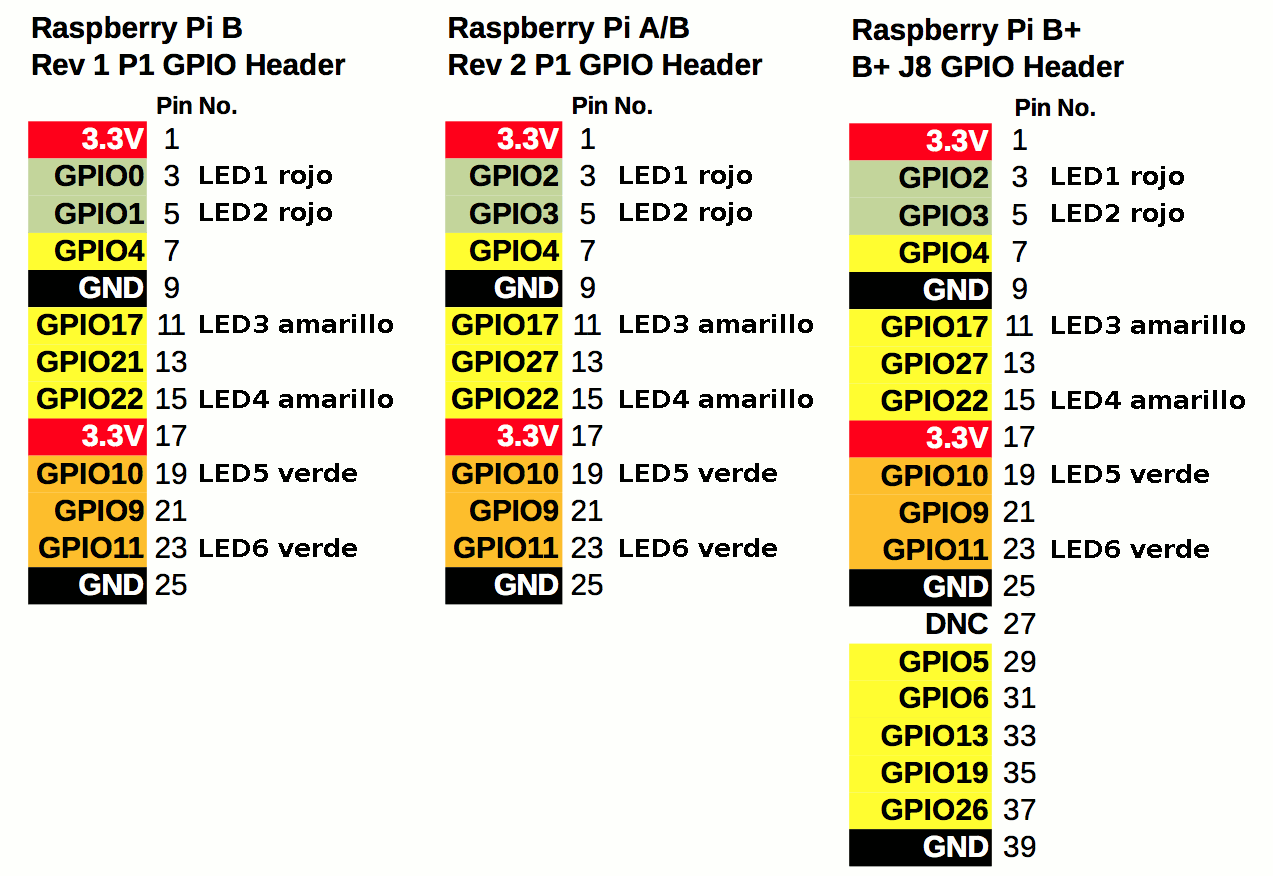
\includegraphics[width=14cm]{graphs/RaspberryGPIOaux.png}
  \caption{Correspondencia LEDs y GPIO}
  \label{fig:pinout2}
\end{figure}

\chapterend
